\Variant{04.10.2026 (1-smena)}
\QQ{1}{$7^{2025}$ sonining önlar xonasidagi raqamini toping.
\Opts{$1$}{$7$}{$0$}{$4$}}
\QQ{2}{Hisoblang: $8{,}0(7)-3{,}1(3)+2{,}0(4)$.
\Opts{$6{,}8(9)$}{$6{,}9(7)$}{$7{,}0(2)$}{$6{,}9(8)$}}
\QQ{3}{Sayyoh $A$ şahardan $B$ şaharga $5$ km/soat tezlik bilan yetib borişni közlab yölga çiqdi. Lekin yölning $\dfrac13$ qismini bosib ötgaç, $20$ minut dam oldi va qolgan yölni $6$ km/soat tezlik bilan bosib, $B$ şaharga öz vaqtida yetib keldi. $A$ va $B$ şaharlar orasidagi masofani toping.
\Opts{$18$}{$12$}{$10$}{$15$}}
\QQ{4}{$A$ va $B$ brigadalar birgalikda işlab, işni $12$ kunda tugatişlari mumkin. Ular $2$ kun birgalikda işlagaç, qolgan işni $B$ brigadaning özi bajardi. $B$ brigadaning mehnat unumdorligi $A$ brigadanikining $66\frac23\%$ ini taşkil etadi. Butun iş neça kunda tugatiladi?
\Opts{$25$}{$22$}{$27$}{$32$}}
\QQ{5}{Hisoblang:
\[\left(\left(3^{-2}\right)^{\frac13}+\left(3^{\frac13}\right)^2+\left(3^2\right)^{\frac13}+\left(3^{\frac13}\right)^{-2}\right)^{\left(\frac13\right)^2-\frac19}\cdot\sqrt{9^3}\]
\Opts{$81$}{$1$}{$27$}{$9$}}
\QQ{6}{Hisoblang: $\sqrt[3]{\sqrt{4096}}-\sqrt{\sqrt[5]{\dfrac1{1024}}}$.
\Opts{$\dfrac{15}4$}{$2$}{$\dfrac72$}{$3$}}
\QQ{7}{Hisoblang:
\[\frac1{2\bigl[\sqrt1\bigr]+1}+\frac1{2\bigl[\sqrt2\bigr]+1}+\frac1{2\bigl[\sqrt3\bigr]+1}+\ldots+\frac1{2\bigl[\sqrt{121}\bigr]+1}\]
Bu yerda $[a]$ — $a$ sonining butun qismi, yaʼni $a$ dan oşmaydigan eng katta butun son.
\Opts{$9\dfrac{22}{23}$}{$10$}{$11\dfrac{22}{23}$}{$10\dfrac1{23}$}}
\QQ{8}{Arifmetik progressiyada $a_8=12$ bölsa, $S_{15}$ ni toping.
\Opts{$90$}{$168$}{$192$}{$180$}}
\QQ{9}{$(a_n)$ arifmetik va $(b_n)$ geometrik progressiyalar uçun $b_1=a_1$, $b_2=a_2$, $b_3=a_1+a_3$ va $b_5=48$ bölsa, $a_1+a_2+a_3+\ldots+a_{10}$ yiğindini toping.
\Opts{$165$}{$180$}{$330$}{$150$}}
\QQ{10}{Agar $\sqrt x+\sqrt y=2$ bölsa,
\[\frac{9x-4y}{3\sqrt x-2\sqrt y}-\sqrt x\]
ifodaning qiymatini toping.
\Opts{$4$}{$8$}{$6$}{$2$}}
\QQ{11}{Ifodani soddalaştiring:
\[\frac1{y(x+z+xyz)}-\frac1{x+\dfrac1{y+\dfrac1z}}:\frac y{xy+1}\]
\Opts{$\dfrac1y$}{$0$}{$1$}{$-1$}}
\QQ{12}{Hisoblang: $\cos405^\circ\cdot\sin315^\circ+\ctg1845^\circ\cdot\ctg585^\circ+\cos720^\circ\cdot\sin810^\circ$.
\Opts{$\dfrac52$}{$\dfrac32$}{$\dfrac12$}{$2$}}
\QQ{13}{$\cos(3x-\pi)=-\sin6x$ tenglamaning eng kiçik musbat ildizini toping.
\Opts{$\dfrac\pi6$}{$\dfrac\pi{18}$}{$\dfrac{5\pi}{18}$}{$\dfrac\pi9$}}
\QQ{14}{Tenglamani yeçing:
\[8^x-\frac8{8^x}-6\left(2^x-\frac1{2^{x-1}}\right)=1\]
\Opts{$2$}{$0$}{$-1$}{$1$}}
\QQ{15}{Tenglamaning haqiqiy ildizlari köpaytmasini toping (agar yagona bölsa, öşa ildizini toping):
\[\sqrt{(2x+1)^2-8x}-2=\sqrt{1-4x}\]
\Opts{$-2$}{$-4$}{$0$}{$2$}}
\QQ{16}{$x-x^2-2x^3=\dfrac13$ tenglama neçta haqiqiy yeçimga ega?
\Opts{$2$ ta}{$3$ ta}{$1$ ta}{haqiqiy ildizga ega emas}}
\QQ{17}{Tenglamalar sistemasi neçta haqiqiy yeçimga ega?
\[\begin{cases}\log_x\sqrt y+\log_yx^2=2,\\ \sqrt y-5\sqrt x=-4\end{cases}\]
\Opts{$2$ ta}{haqiqiy yeçimga ega emas}{$1$ ta}{$3$ ta}}
\QQ{18}{Tengsizlik neçta butun yeçimga ega?
\[\frac1{\sqrt{x+6}}-\frac1{3-x}\le0\]
\Opts{$1$ ta}{$2$ ta}{$3$ ta}{çeksiz köp}}
\QQ{19}{$x\in[-20;\,20]$ bölsa, neçta butun son tengsizlikni qanoatlantiradi?
\[\sqrt{x^2-10x+16}<2x-4\]
\Opts{$13$ ta}{$14$ ta}{$38$ ta}{$19$ ta}}
\QQ{20}{Çiziqli funksiya grafigi koordinatalar boşidan va $(-2;\,3)$ nuqtadan ötadi. Funksiya grafigi qaysi çoraklarda yotadi?
\Opts{II, IV}{I, III}{I, II}{III, IV}}
\QQ{21}{$f(2x-2)=6x-5$ va $f\bigl(g(x)\bigr)=x^2$ bölsa, $g(2)$ ni toping.
\Opts{$1$}{$\dfrac13$}{$3$}{$2$}}
\QQ{22}{Rasmda $y=f(x)$ funksiyaning $[a;\,b]$ kesmadagi hosilasining grafigi tasvirlangan. Uşbu oraliqda $f(x)$ funksiyaning neçta lokal maksimum nuqtasi bor?
\qfig{\begin{tikzpicture}[xscale=0.75,yscale=1.05,font=\small]
\draw[-{Stealth[length=4pt]}] (-5.6,0)--(5.8,0) node[right] {$x$}; \draw[-{Stealth[length=4pt]}] (0,-1.5)--(0,2.1) node[left] {$y$};
\draw[thick] plot[smooth] coordinates {(-5.00,-1.000) (-4.90,-0.826) (-4.80,-0.643) (-4.70,-0.460) (-4.60,-0.286) (-4.50,-0.130) (-4.40,-0.000) (-4.30,0.114) (-4.20,0.229) (-4.10,0.343) (-4.00,0.455) (-3.90,0.564) (-3.80,0.668) (-3.70,0.767) (-3.60,0.858) (-3.50,0.942) (-3.40,1.015) (-3.30,1.079) (-3.20,1.130) (-3.10,1.168) (-3.00,1.192) (-2.90,1.200) (-2.80,1.184) (-2.70,1.139) (-2.60,1.069) (-2.50,0.978) (-2.40,0.870) (-2.30,0.750) (-2.20,0.622) (-2.10,0.489) (-2.00,0.356) (-1.90,0.228) (-1.80,0.108) (-1.70,0.000) (-1.60,-0.114) (-1.50,-0.244) (-1.40,-0.375) (-1.30,-0.489) (-1.20,-0.569) (-1.10,-0.600) (-1.00,-0.590) (-0.90,-0.561) (-0.80,-0.517) (-0.70,-0.458) (-0.60,-0.389) (-0.50,-0.310) (-0.40,-0.225) (-0.30,-0.136) (-0.20,-0.045) (-0.10,0.053) (-0.00,0.199) (0.10,0.383) (0.20,0.589) (0.30,0.797) (0.40,0.990) (0.50,1.150) (0.60,1.260) (0.70,1.300) (0.80,1.001) (0.90,0.413) (1.00,0.000) (1.10,-0.162) (1.20,-0.299) (1.30,-0.406) (1.40,-0.475) (1.50,-0.500) (1.60,-0.469) (1.70,-0.386) (1.80,-0.270) (1.90,-0.135) (2.00,-0.000) (2.10,0.168) (2.20,0.396) (2.30,0.659) (2.40,0.930) (2.50,1.185) (2.60,1.399) (2.70,1.545) (2.80,1.600) (2.90,1.585) (3.00,1.541) (3.10,1.472) (3.20,1.381) (3.30,1.271) (3.40,1.146) (3.50,1.010) (3.60,0.865) (3.70,0.714) (3.80,0.562) (3.90,0.411) (4.00,0.265) (4.10,0.127) (4.20,0.000) (4.30,-0.121) (4.40,-0.244) (4.50,-0.369) (4.60,-0.495) (4.70,-0.621) (4.80,-0.748) (4.90,-0.874) (5.00,-1.000)};
\draw[dashed] (-5,0)--(-5,-1); \draw[dashed] (5,0)--(5,-1); \node[above] at (-5,0) {$a$}; \node[above] at (5,0) {$b$}; \node[right] at (3.1,1.6) {$f'(x)$};
\end{tikzpicture}}
\Opts{$2$ ta}{$3$ ta}{$4$ ta}{$6$ ta}}
\QQ{23}{Integralni hisoblang:
\[\int\limits_0^{\frac\pi2}\frac{\cos x}{\cos^2x+15}\,dx\]
\Opts{$\ln\sqrt[8]{\dfrac35}$}{$\ln\sqrt[4]{\dfrac53}$}{$\ln\sqrt[8]{15}$}{$\ln\sqrt[8]{\dfrac53}$}}
\QQ{24}{Radiuslari $2$ va $5$ bölgan ikki aylana taşqi tomondan urinadi. Ularning umumiy taşqi urinmasi aylanalarga $A$ va $B$ nuqtalarda urinadi. $AB$ ni toping.
\qfig{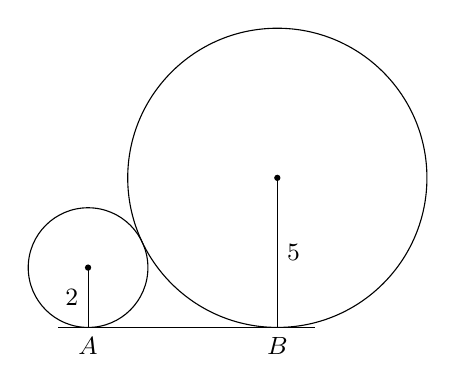
\begin{tikzpicture}[scale=0.38,font=\small]
\draw (0,2) circle (2); \draw (6.325,5) circle (5); \draw (-1,0)--(7.6,0); \draw (0,0)--(0,2); \draw (6.325,0)--(6.325,5);
\fill (0,2) circle (3pt); \fill (6.325,5) circle (3pt); \node[left] at (0,1) {$2$}; \node[right] at (6.325,2.5) {$5$};
\node[below] at (0,0) {$A$}; \node[below] at (6.325,0) {$B$};
\end{tikzpicture}}
\Opts{$3\sqrt5$}{$2\sqrt{10}$}{$7$}{$\sqrt{10}$}}
\QQ{25}{Uçburçakning $B$ va $C$ uçlaridagi taşqi burçaklari yiğindisi $A$ burçakdan $3$ marta katta. $AC=4$, $AB=5$ bölsa, uçburçak yuzini toping.
\Opts{$10\sqrt3$}{$10$}{$5\sqrt3$}{$20$}}
\QQ{26}{Teng yonli $ABC$ uçburçakka ($AB=BC$) radiusi $4$ ga teng aylana içki çizilgan. Radiusi $1$ ga teng aylana $AB$ va $BC$ tomonlarga hamda birinçi aylanaga taşqi tomondan urinadi. Uçburçakning $AC$ asosini toping.
\qfig{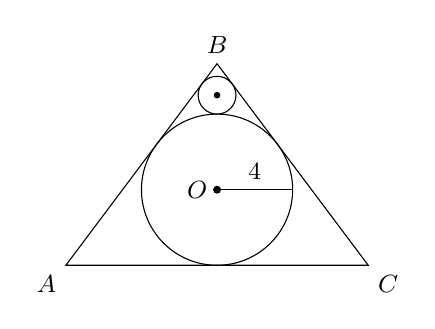
\begin{tikzpicture}[scale=0.24,font=\small]
\coordinate (A) at (-8,0); \coordinate (C) at (8,0); \coordinate (B) at (0,10.667);
\draw (A)--(B)--(C)--cycle; \draw (0,4) circle (4); \draw (0,9) circle (1); \fill (0,4) circle (6pt); \fill (0,9) circle (5pt);
\draw (0,4)--(4,4); \node[above] at (2,4) {$4$}; \node[left] at (0,4) {$O$};
\node[below left] at (A) {$A$}; \node[above] at (B) {$B$}; \node[below right] at (C) {$C$};
\end{tikzpicture}}
\Opts{$8$}{$10$}{$16$}{$12$}}
\QQ{27}{$ABCD$ parallelogrammning $A$ va $D$ burçak bissektrisalari ötkazilgan bölib, ular $E$ nuqtada kesişadi. Agar parallelogrammning yuzi $48$ ga teng bölsa, böyalgan $ABE$ uçburçak yuzini toping.
\qfig{\begin{tikzpicture}[scale=0.62,font=\small]
\coordinate (A) at (0,0); \coordinate (B) at (5.6,0); \coordinate (C) at (7.6,3.4); \coordinate (D) at (2,3.4); \coordinate (E) at (2.974,1.700);
\fill[qfill] (A)--(B)--(E)--cycle;
\draw (A)--(B)--(C)--(D)--cycle; \draw (A)--(E)--(B); \draw (D)--(E);
\node[below left] at (A) {$A$}; \node[below right] at (B) {$B$}; \node[above right] at (C) {$C$}; \node[above left] at (D) {$D$}; \node[above right] at (E) {$E$};
\end{tikzpicture}}
\Opts{$10$}{$12$}{$16$}{$8$}}
\QQ{28}{Muntazam oltiburçakning yuzi $54\sqrt3$ ga teng. Oltiburçakka içki va taşqi çizilgan aylanalar orasidagi yuzani toping.
\qfig{\begin{tikzpicture}[scale=0.3,font=\small]
\fill[qfill,even odd rule] (0,0) circle (6) (0,0) circle (5.196);
\draw (0,0) circle (6); \draw (0,0) circle (5.196);
\draw (240:6)--(300:6)--(0:6)--(60:6)--(120:6)--(180:6)--cycle;
\foreach \n/\a in {A/240,B/300,C/0,D/60,E/120,F/180} \node at (\a:7) {$\n$};
\end{tikzpicture}}
\Opts{$12\pi$}{$6\pi$}{$9\pi$}{$15\pi$}}
\QQ{29}{Asoslari $16$ va $30$ bölgan teng yonli trapetsiya berilgan. Trapetsiya tekisligidan taşqaridagi nuqtadan uning barça tomonlarigaça bölgan masofalar $11$ ga teng. Şu nuqtadan trapetsiya tekisligigaça bölgan masofani toping.
\Opts{$1$}{$3$}{$2$}{$\sqrt{11}$}}
\QQ{30}{$7x+24y=168$ töğri çiziqdan koordinatalar boşigaça bölgan eng qisqa masofani toping.
\Opts{$6\dfrac{18}{25}$}{$6\dfrac3{25}$}{$6\dfrac12$}{$8\dfrac25$}}
\QQ{31}{$A=\{a;\,b;\,d;\,f;\,g;\,k\}$, $B=\{a;\,b;\,f;\,g;\,m\}$ va $C=\{a;\,b;\,f;\,g;\,n;\,p\}$ töplamlar berilgan. $(A\cap B)\cup C$ töplam neçta elementdan iborat?
\Opts{$12$}{$4$}{$6$}{$2$}}
\QQ{32}{$3$ ta kubik bir vaqtda taşlanganda, uçalasida ham bir xil son tuşiş ehtimolligini toping.
\Opts{$\dfrac1{36}$}{$\dfrac16$}{$\dfrac1{216}$}{$\dfrac1{18}$}}
\QQ{33}{\Moslash{Radiusi $6$ ga, markaziy burçagi $60^\circ$ ga teng $AOB$ sektor berilgan, $OC$ — uning bissektrisasi. $A$ va $C$ nuqtalardan $OB$ ga $AD$ va $CF$ perpendikulyarlar tuşirilgan. Sektorni örab konus yasalgan, konusga şar içki çizilgan.
\par\centering\begin{tikzpicture}[scale=0.42,font=\small]
\coordinate (O) at (0,0); \coordinate (B) at (6,0); \coordinate (A) at (3,5.196); \coordinate (C) at (5.196,3); \coordinate (D) at (3,0); \coordinate (F) at (5.196,0);
\fill[qfill] (D)--(A) arc (60:30:6)--(F)--cycle;
\draw (O)--(B) arc (0:60:6)--cycle; \draw (O)--(C); \draw (A)--(D); \draw (C)--(F);
\draw (1.1,0) arc (0:30:1.1); \draw (1.5,0.866) arc (30:60:1.73); \node at (1.95,0.45) {\tiny$30^\circ$}; \node at (1.4,1.55) {\tiny$30^\circ$};
\node[left] at (O) {$O$}; \node[below] at (D) {$D$}; \node[below] at (F) {$F$}; \node[below right] at (B) {$B$}; \node[above] at (A) {$A$}; \node[above right] at (C) {$C$}; \node[above left] at (1.5,2.6) {$6$};
\begin{scope}[xshift=9.5cm]
\draw (-1.6,0)--(0,5.6)--(1.6,0); \draw (-1.6,0) arc (180:360:1.6 and 0.4); \draw[dashed] (1.6,0) arc (0:180:1.6 and 0.4);
\draw (0,1.25) circle (1.25); \fill (0,1.25) circle (3pt); \draw[dashed] (0,0)--(1.6,0); \node[below] at (0.8,-0.4) {$R$};
\end{scope}
\end{tikzpicture}}{A) $3\pi$\par B) $\dfrac{128\pi}{49}$\par C) $12\pi$\par D) $27\pi$\par E) $7\pi$\par F) $\dfrac{20\pi}7$}{Böyalgan soha yuzini toping.}{Konusning töla sirtini toping.}{Konusga içki çizilgan şar sirtining yuzini toping.}}
\QQ{36}{Tenglama berilgan:
\[\frac{x^4-2x^3}{x-2}-\frac{9x^2+18x}{x+2}=a\]
\AB{Tenglama ikkita yeçimga ega böladigan $a$ ning qiymatlari sonini toping.}{Tenglama ikkita yeçimga ega böladigan $a$ ning eng katta qiymatini toping.}}
\QQ{37}{Tenglama berilgan:
\[\frac1{2\tg^2x+1}+\frac1{2\ctg^2x+1}=\frac{30\cos4x}{8+\sin^22x}\]
\AB{Tenglamaning $\left[-\dfrac\pi2;\,\dfrac{3\pi}2\right]$ kesmadagi ildizlari sonini toping.}{Tenglamaning $(0;\,2\pi)$ oraliqdagi ildizlari yiğindisini toping.}}
\QQ{38}{$f(x)=ax^2+bx+c$ va $g(x)=k\sqrt{x+l}$ funksiyalar berilgan. $f$ funksiyaning grafigi $Ox$ öqini $(m;\,0)$ va $(5;\,0)$ nuqtalarda kesib ötadi, parabolaning uçi esa $(2;\,-4{,}5)$ nuqtada joylaşgan. $f$ va $g$ funksiyalarning grafiklari $(m;\,0)$ va $(0;\,n)$ nuqtalarda kesişadi.
\qfig{\begin{tikzpicture}[xscale=0.55,yscale=0.4,font=\small]
\draw[-{Stealth[length=4pt]}] (-2.2,0)--(6.5,0) node[right] {$x$}; \draw[-{Stealth[length=4pt]}] (0,-6.5)--(0,3.3) node[left] {$y$};
\draw[thick,domain=-1.9:5.65,samples=80] plot (\x,{0.5*\x*\x-2*\x-2.5}); \draw[thick,domain=-1:6,samples=100] plot (\x,{-2.5*sqrt(\x+1)});
\foreach \p in {(-1,0),(5,0),(0,-2.5),(2,-4.5)} \fill \p circle (2.5pt);
\node[above left] at (-1,0) {\scriptsize$(m;\,0)$}; \node[above right] at (5,0) {\scriptsize$(5;\,0)$}; \node[left] at (0,-2.5) {\scriptsize$(0;\,n)$}; \node[below] at (2,-4.7) {\scriptsize$(2;\,-4{,}5)$};
\node[right] at (5.65,3.1) {$f(x)$}; \node[right] at (6,-6.6) {$g(x)$};
\end{tikzpicture}}
\AB{$f(-2)$ ning qiymatini toping.}{$\dfrac{a-b-l-c}{k-m-n}$ ifodaning qiymatini toping.}}
\QQ{39}{$f(3)=15$, $f'(3)=13$, $f'(7)=2$, $g(3)=7$, $g'(3)=6$, $g(7)=3$ va $g'(7)=0$ ekanligi maʼlum.
\AB{$h(x)=f\bigl(g(x)\bigr)$ bölsa, $h'(3)$ ni toping.}{$k(x)=\dfrac{f(x)}{g(x)}$ bölsa, $k'(7)$ ni toping.}}
\QQ{40}{Çizmada $y=ax^2+bx+c$ parabola va $y=kx+l$ töğri çiziq grafiklari tasvirlangan. Parabola abssissalar öqini $x=-1$ va $x=4$ nuqtalarda kesib ötadi. Töğri çiziq esa parabolaga $M(3;\,8)$ nuqtada urinadi.
\qfig{\begin{tikzpicture}[xscale=0.62,yscale=0.2,font=\small]
\fill[qfill] (-1,0)--plot[domain=-1:0,samples=30] (\x,{-2*\x*\x+6*\x+8})--(0,0)--cycle;
\fill[qfill] (3,8)--plot[domain=3:4,samples=30] (\x,{-2*\x*\x+6*\x+8})--(4.333,0)--cycle;
\draw[-{Stealth[length=4pt]}] (-2,0)--(6,0) node[right] {$x$}; \draw[-{Stealth[length=4pt]}] (0,-3.5)--(0,15.5) node[left] {$y$};
\draw[thick,domain=-1.3:4.55,samples=80] plot (\x,{-2*\x*\x+6*\x+8}); \draw[thick] (2.2,12.8)--(4.85,-3.1);
\fill (3,8) circle (3.5pt); \node[right] at (3.1,8.4) {\scriptsize$M(3;\,8)$};
\node[below left] at (-1,0) {\scriptsize$-1$}; \node[below left] at (4,0) {\scriptsize$4$};
\node[left] at (-0.9,10) {\scriptsize$y=ax^2+bx+c$}; \node[right] at (4.85,-3.1) {\scriptsize$y=kx+l$};
\end{tikzpicture}}
\AB{$\dfrac{a+b+c}{k-l}$ ifodaning qiymatini hisoblang.}{Böyalgan sohaning yuzini toping.}}
\QQ{41}{$ABC$ töğri burçakli uçburçakda $\angle A=90^\circ$. $BD$ — $B$ burçak bissektrisasi, $BD\perp ED$ ($E\in BC$). $AD=4$ va $BE=3EC$ ekanligi maʼlum.
\qfig{\begin{tikzpicture}[scale=0.42,font=\small]
\coordinate (A) at (0,0); \coordinate (B) at (0,8); \coordinate (C) at (10.667,0); \coordinate (D) at (4,0); \coordinate (E) at (8,2);
\fill[qfill] (B)--(D)--(E)--cycle;
\draw (A)--(B)--(C)--cycle; \draw (B)--(D)--(E); \draw (0,0.5)--(0.5,0.5)--(0.5,0);
\node[left] at (A) {$A$}; \node[left] at (B) {$B$}; \node[right] at (C) {$C$}; \node[below] at (D) {$D$}; \node[above right] at (E) {$E$}; \node[below] at (2,0) {$4$};
\end{tikzpicture}}
\AB{$DE$ kesma uzunligini toping.}{$BED$ uçburçak yuzini toping.}}
\QQ{42}{$ABCD$ törtburçakda $AB=AD=13$ sm va $BC=CD=15$ sm. Törtburçakning kiçik diagonali diagonallar kesişiş nuqtasidan $5:9$ nisbatda bölinadi.
\AB{$ABCD$ törtburçak yuzini toping.}{Içki çizilgan aylana markazidan diagonallar kesişiş nuqtasigaça bölgan masofani toping.}}
\QQ{43}{Burçaklari bir xil bölgan $ABCDEF$ oltiburçak berilgan. $AB=4$, $BC=6$, $CD=10$, $FE=2$.
\AB{$DE$ tomonni toping.}{$ABCDEF$ oltiburçakning yuzini toping.}}
\QQ{44}{Silindrga konus içki çizilgan bölib, ular asosdoş, konus uçi silindrning ustki asosi markazida yotadi. Silindr asosi diametrining balandligiga nisbati $3:2$ ga teng. Konusdan ortib qolgan böşliqqa silindrning yon sirti, ustki asosi va konusning yon sirtiga urinadigan şar joylaştirilgan.
\qfig{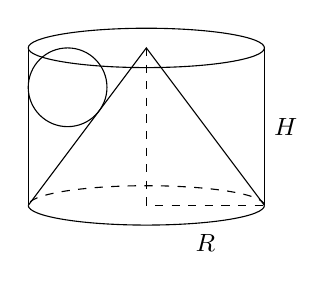
\begin{tikzpicture}[scale=0.5,font=\small]
\draw (0,4) ellipse (3 and 0.5); \draw (-3,0)--(-3,4); \draw (3,0)--(3,4); \draw (-3,0) arc (180:360:3 and 0.5); \draw[dashed] (3,0) arc (0:180:3 and 0.5);
\draw (-3,0)--(0,4)--(3,0); \draw[dashed] (0,4)--(0,0)--(3,0); \draw (-2,3) circle (1);
\node[right] at (3,2) {$H$}; \node[below] at (1.5,-0.5) {$R$};
\end{tikzpicture}}
\AB{Konus hajmining şar hajmiga nisbatini toping.}{Agar şarning töla sirti $4\pi$ ga teng bölsa, silindr hajmini toping.}}
\QQ{45}{Ustki qopqoği bölmagan $8\pi$ litr hajmli silindr şaklidagi idişni eng kam miqdordagi listdan tayyorlaş kerak. $1\text{ m}^2$ list narxi $150\,000$ söm.
\AB{Idişning balandligini (sm da) toping.}{Idiş uçun qança xarajat qilinadi ($\pi=3$ deb oling)?}}
\Javoblar{C D D C C C D D A A D B B D A C C B A A A B D B B C B C A A C A A E F}{\OK{36}{$4$}{$6\sqrt3$}\OK{37}{$8$}{$8\pi$}\OK{38}{$3{,}5$}{$4$}\OK{39}{$12$}{$\dfrac23$}\OK{40}{$-\dfrac38$}{$\dfrac{16}3$}\OK{41}{$2\sqrt5$}{$20$}\OK{42}{$168$}{$1{,}5$}\OK{43}{$8$}{$70\sqrt3$}\OK{44}{$9$}{$36\pi$}\OK{45}{$20$ sm}{$54\,000$ söm}}
